\documentclass{article}
\usepackage[utf8]{inputenc}
\usepackage[T1]{fontenc}
\usepackage{geometry}
\usepackage{graphicx}

\geometry{margin=0.5in}

\begin{document}

\section*{Task}
You need to write and run a program that measures time with a resolution of \textbf{1 second} and displays the counted value on 7-segment displays (P2). \\
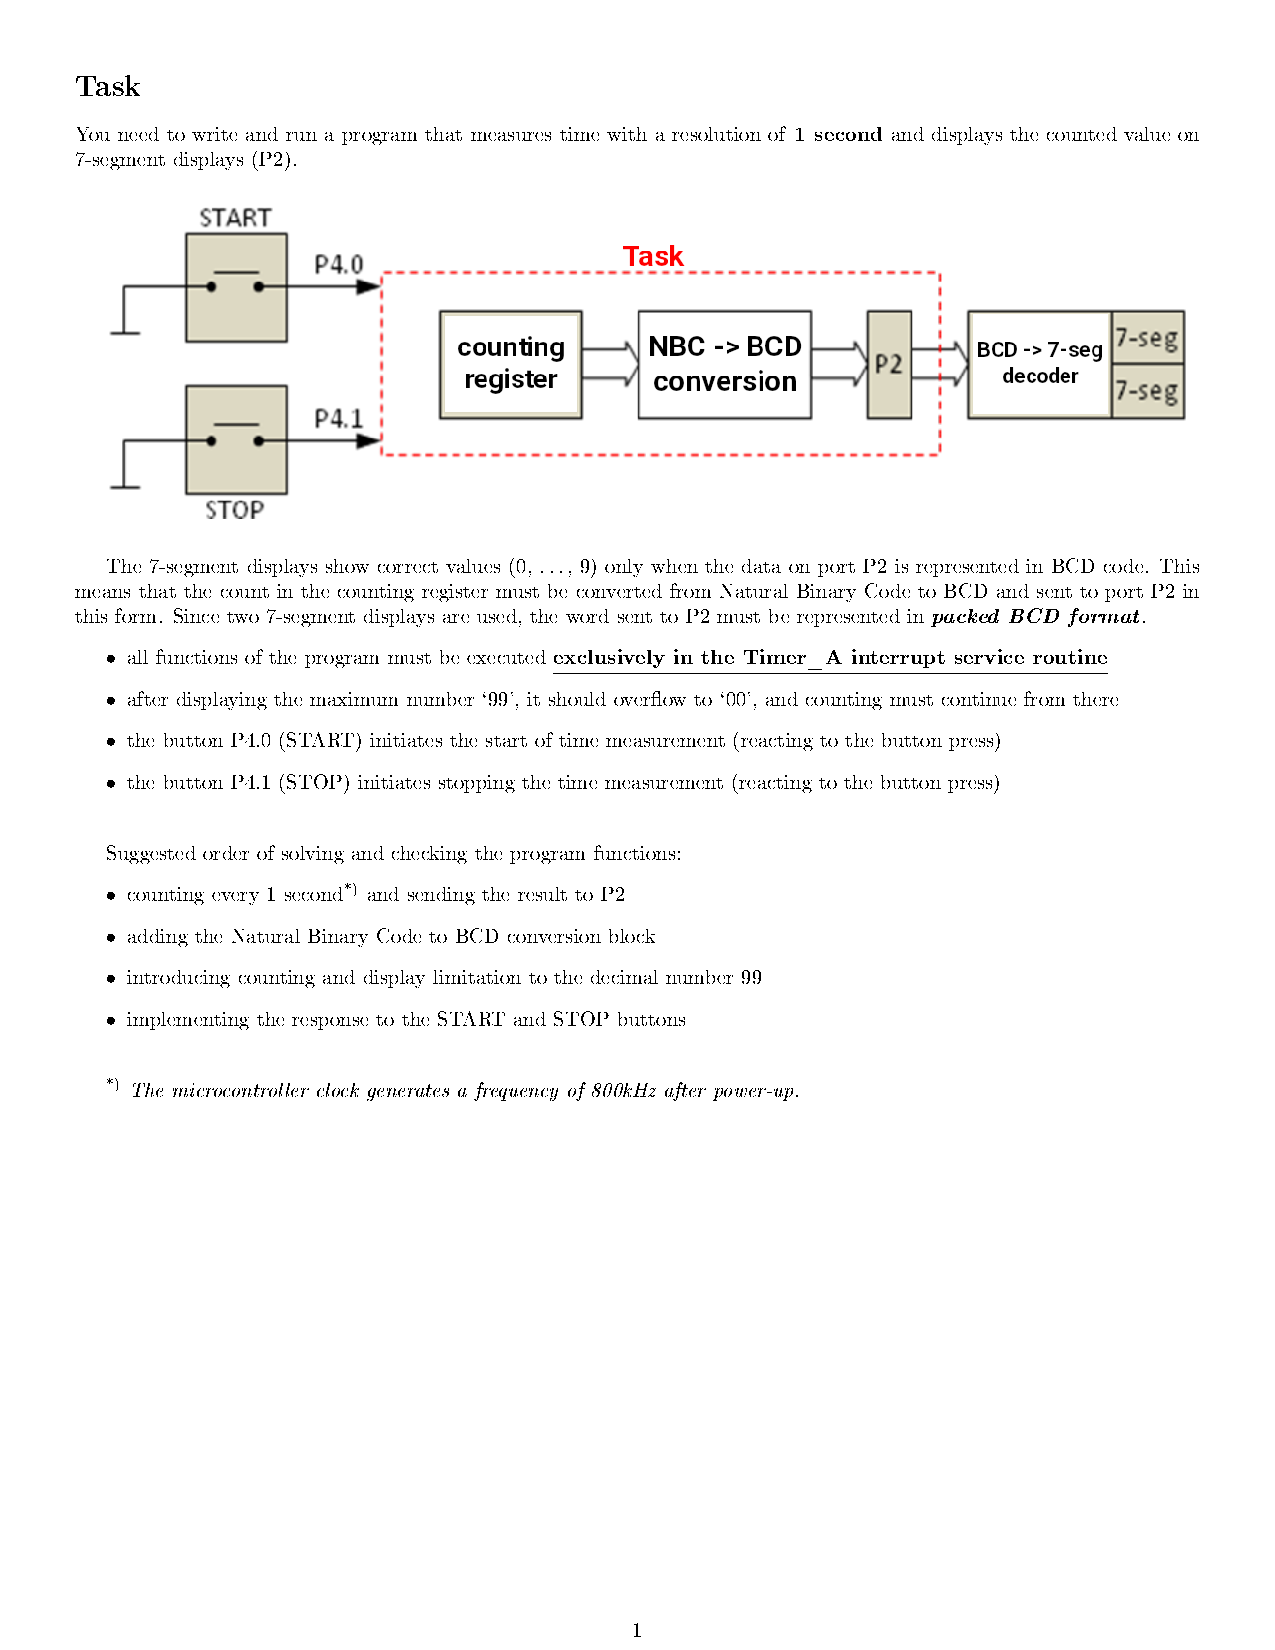
\includegraphics[width=\textwidth]{"../img/TIMER_A_NBC2BCD_2.png"}

The 7-segment displays show correct values (0, …, 9) only when the data on port P2 is represented in BCD code. This means that the count in the counting register must be converted from Natural Binary Code to BCD and sent to port P2 in this form. Since two 7-segment displays are used, the word sent to P2 must be represented in \textbf{\textit{packed BCD format}}.
\begin{itemize}
    \item all functions of the program must be executed \textbf{\underline{exclusively in the Timer\_A interrupt service routine}}
    \item after displaying the maximum number \textquoteleft99\textquoteright, it should overflow to \textquoteleft00\textquoteright, and counting must continue from there
    \item the button P4.0 (START) initiates the start of time measurement (reacting to the button press)
    \item the button P4.1 (STOP) initiates stopping the time measurement (reacting to the button press)
\end{itemize}
\vspace{5mm}

Suggested order of solving and checking the program functions:
\begin{itemize}
    \item counting every 1 second\textsuperscript{*)} and sending the result to P2
    \item adding the Natural Binary Code to BCD conversion block
    \item introducing counting and display limitation to the decimal number 99
    \item implementing the response to the START and STOP buttons
\end{itemize}
\vspace{5mm}

\textsuperscript{*)} \textit{The microcontroller clock generates a frequency of 800kHz after power-up.}

\end{document}